\chapter{Trigonometry}

In the first half of this chapter the three trigonometric functions (sine, cosine and tangent) will be viewed as functions of angles. The second half of the chapter will approach trigonometry as functions of real numbers.

%---------------------------------------------------
% the unit circle and radians
%---------------------------------------------------
\section{The Unit Circle}
The convention for measuring angles can be seen in the diagram below, beginning from the positive $x$-axis and rotating a point from $(1,0)$ counter-clockwise through $(x,y)$. This traces out an angle, $\theta$. The relationship between the angle and the arc length defines a radian. When the arc length equals the radius, the angle $\theta=1$ radian. The convention is that the positive direction for measuring angles is anticlockwise and the negative direction for measuring angles is clockwise. This setup also defines a right-angled triangle with hypotenuse $r$. As the radius rotates, all the different right-triangles are drawn. See the \href{https://www.desmos.com/calculator/4t6zc5eucd}{link} for the animated version.

\begin{figure}[h]
	\begin{center}
		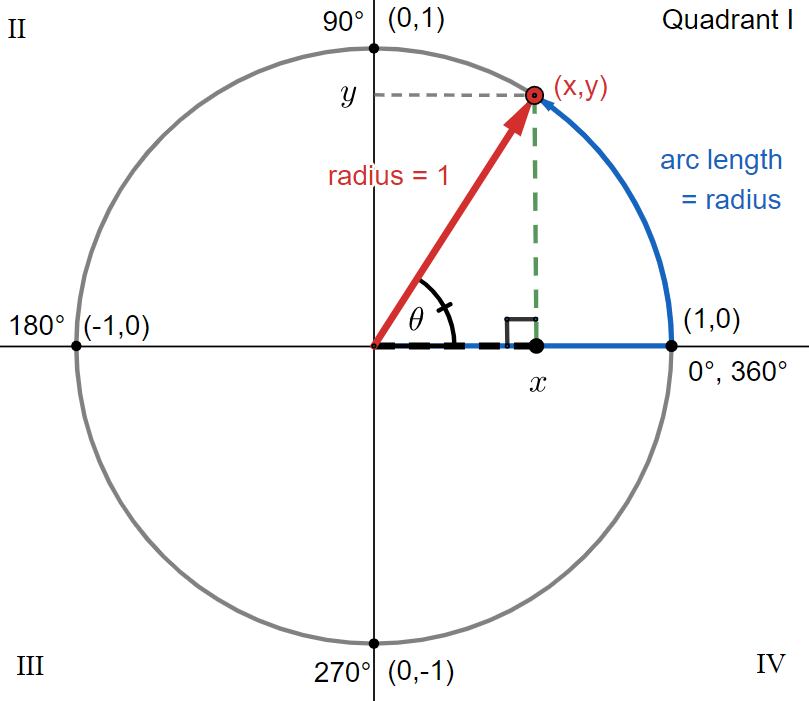
\includegraphics[width=12cm]{unitCircle}
		\caption{The unit circle has a radius of 1. When the arc length from $(1,0)$ to $(x,y)$ is equal to the radius, the angle $\theta$ is 1 radian. There are $2\pi$ radians in one complete rotation. Click \href{https://www.desmos.com/calculator/4t6zc5eucd}{here} for an animated version in Desmos.}
		\label{fig:unitCircle}
	\end{center}
\end{figure}

\subsection*{Relationship between Degrees and Radians}
The abbreviation for radians is \textit{rad}. One complete revolution is \ang{360} which is equivalent to $2 \pi $ radians. It will help to remember one of these conversion factors:
\begin{tcolorbox}\[1\text{ rev }=2\pi \text{ radians} =  \ang{360} \qquad\text{ or }\qquad\pi \text{ radians} =  \ang{180}\]
\end{tcolorbox}

\example\medskip\\
(a) Convert \ang{36} to radians\hspace{0.7cm} 
(b) Convert $\displaystyle\frac{\pi }{3}$ $\mbox{rad}$ to degrees \hspace{0.7cm} 
(c) Convert $1$ $\mbox{rad}$ to degrees \medskip\\

\solution Begin with the conversion factor and then modify as necessary.
\begin{tasks}[before-skip = {0ex} , after-skip={-5ex}](3)
\task \begin{align*}\ang{180}  &  =  \pi \text{ rad} \\
\ang{1}  &  =  \frac{\pi }{180}\text{ rad} \\
\ang{1} \times 36 &  =  \frac{\pi }{180} \times 36 =\frac{\pi }{5}\text{ rad}\end{align*}
\task
\begin{align*}\pi  \text{ rad} &  =  \ang{180}  \\
\frac{\pi }{3} \text{ rad} &  = \frac{\ang{180} }{3} =\ang{60} \end{align*}
\task
\begin{align*}\pi  \text{ rad} &  =  \ang{180} \\
1 \text{ rad} &  =  \frac{\ang{180} }{\pi } \\
 &  \approx   \ang{57.3} \end{align*}
\end{tasks}
Note the similarity between the answers to (b) and (c). This is because $\frac{\pi }{3} =1.0472$ so you would expect the values in degrees to be similar. Always include units with your angle whether they be degrees, radians, or even \textit{gradians}. There are 400 gradians in a circle. This unit is not often used, however, your calculator supports all three.\\
\begin{figure}[h]
\begin{center}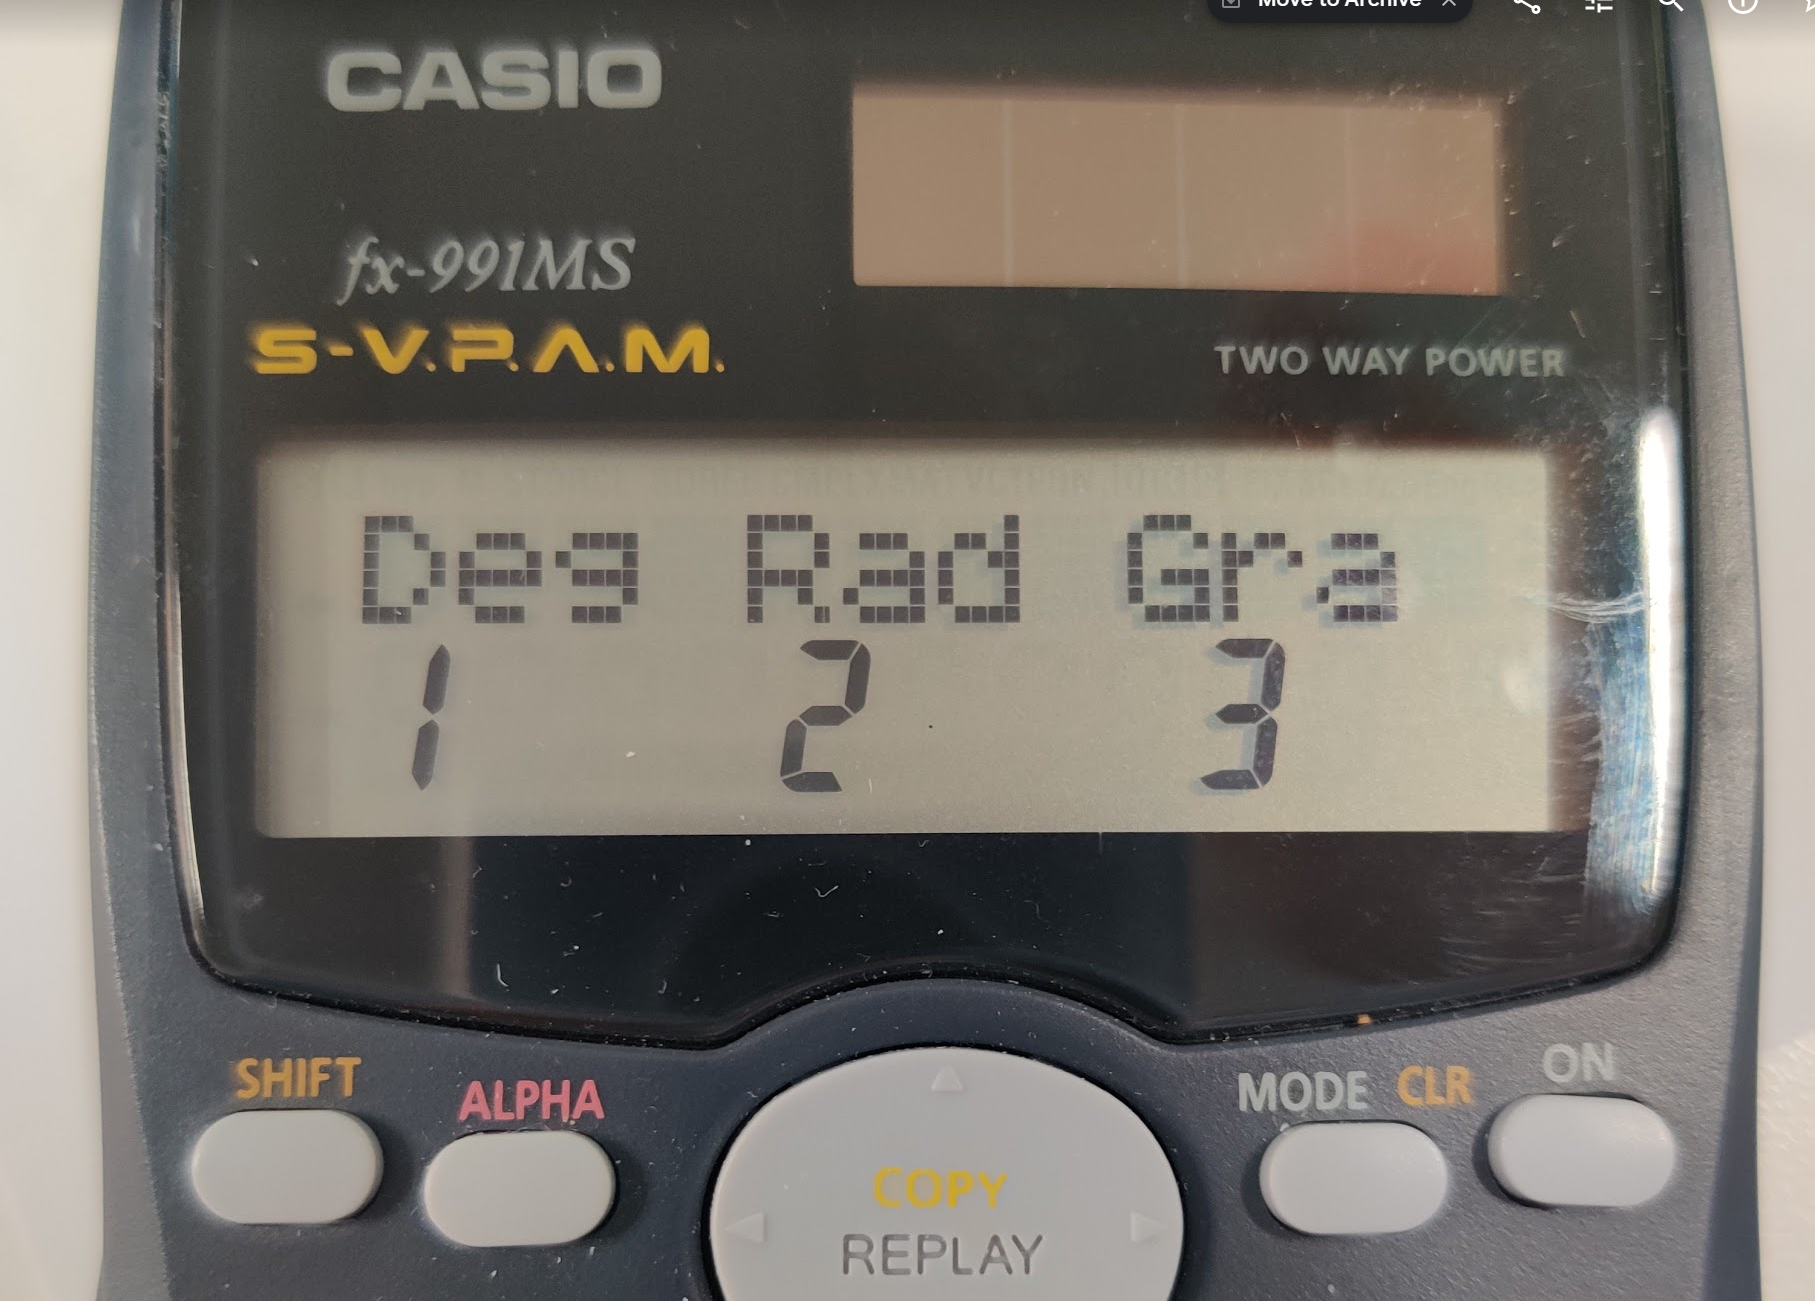
\includegraphics[width=6cm]{calculator1}\hspace{1cm}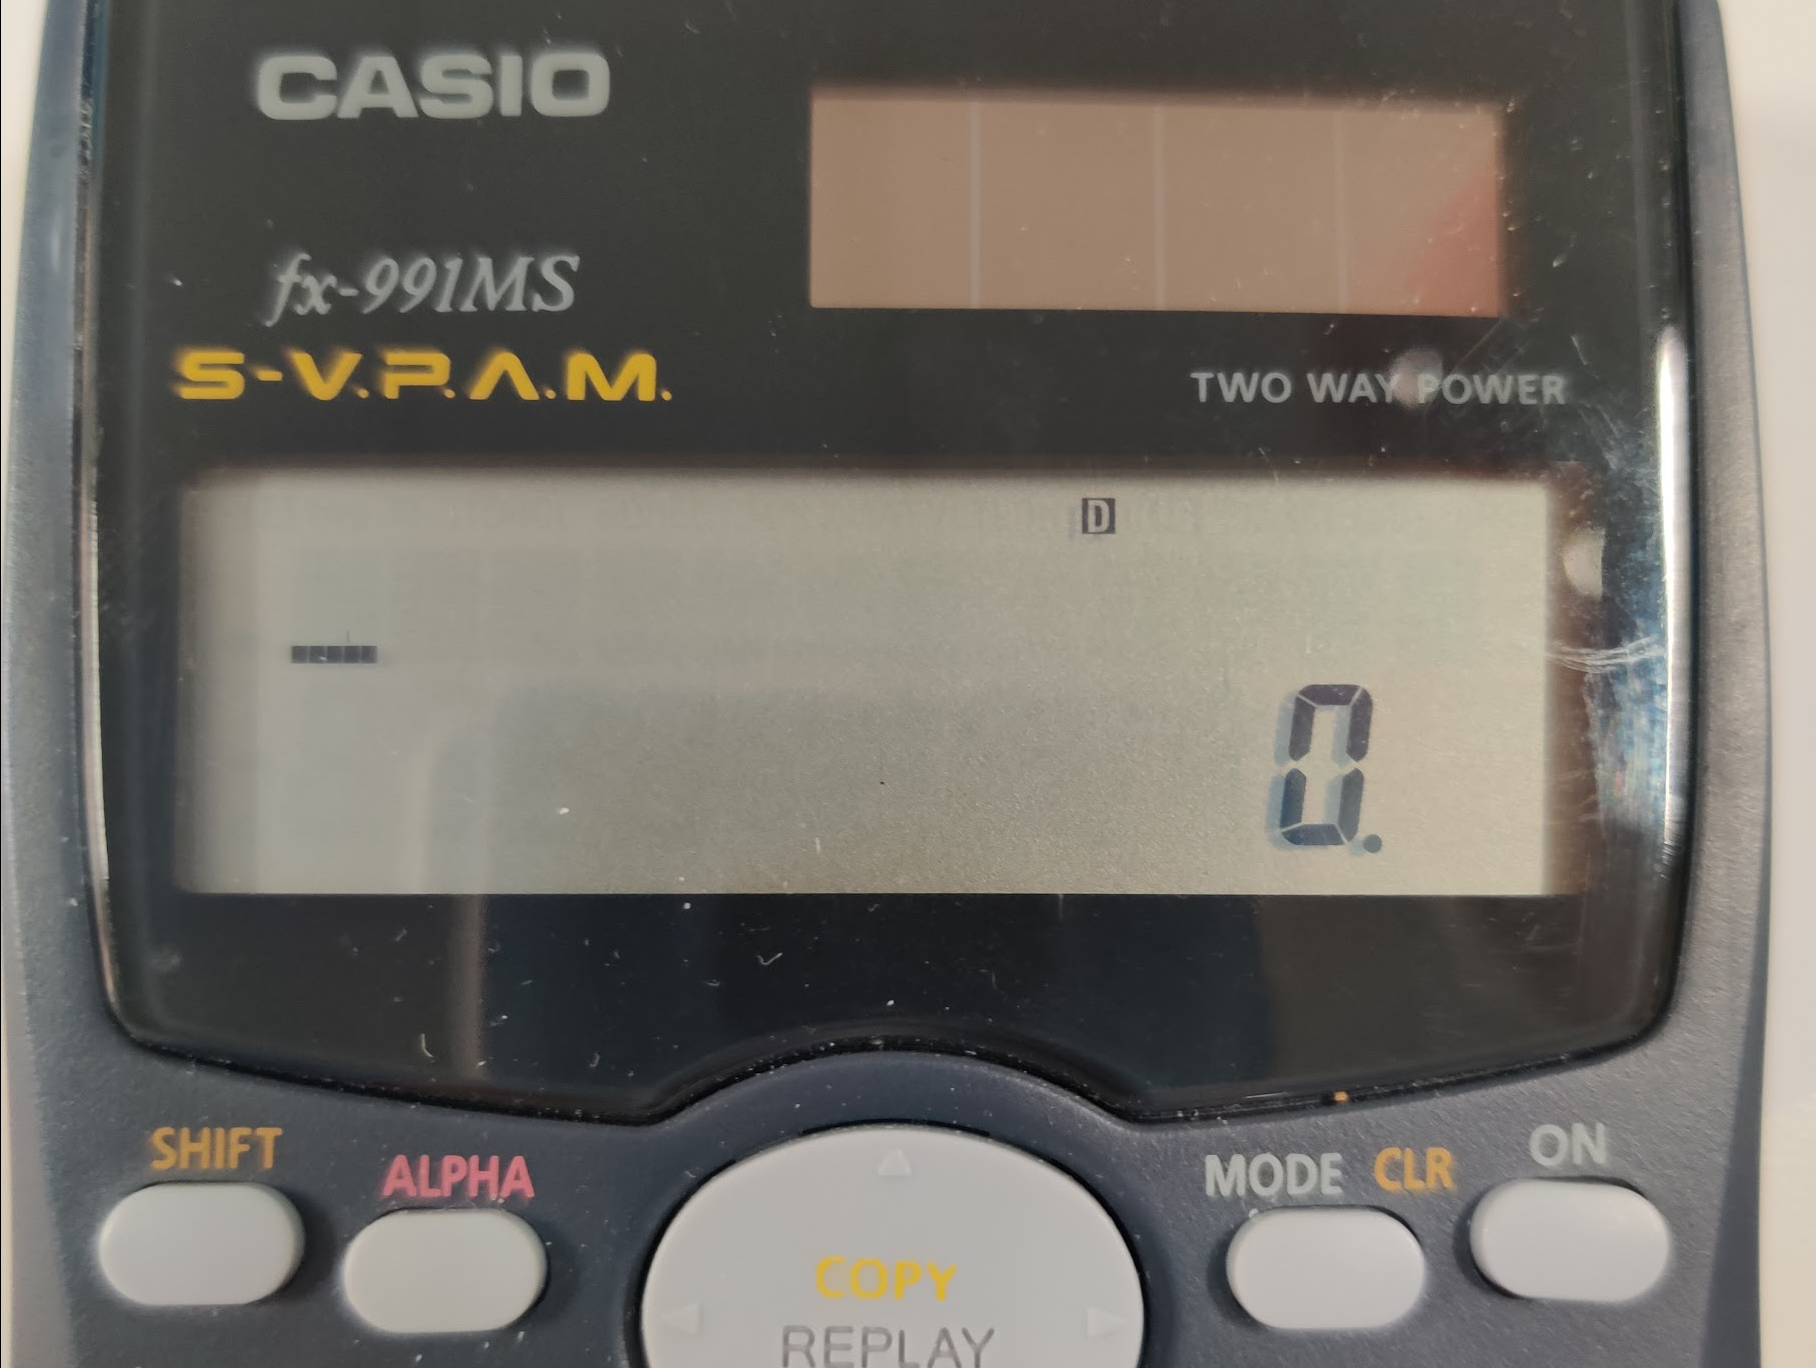
\includegraphics[width=6.8cm]{calculator2}\end{center}
\caption{Your calculator can switch between degrees, radians, and gradians. On the right is a `D' indicating degree mode.}
\end{figure}

\subsection*{Arc Length}
Let $\theta $ be the angle subtended at the centre for the ends of an arc of any circle then the fraction of the circumference of the circle is $\frac{\theta }{2 \pi }$ if $\theta $ is measured in radians and $\frac{\theta }{\ang{360}}$ if $\theta $ is measured in degrees. The length of the circumference of any circle whose radius is $r$ is $2 \pi  r$. If $\theta $ is measured in radians
\begin{equation*}\text{length of arc} =\frac{\theta }{2 \pi } \times 2 \pi  r =\theta  r
\end{equation*}
And if $\theta $ is measured in degrees
\begin{equation*}\text{length of arc} =\frac{\theta }{\ang{360}} \times 2 \pi  r
\end{equation*}
\example Find the length of an arc that subtends an angle of \ang{45} at the centre of a circle whose radius is 9 cm. 

\solution \begin{tasks}[counter-format=(tsk[1]),before-skip = {0ex},after-skip={-5ex}](2)
	\task Method 1:\begin{eqnarray*}\text{Length of arc} &  = & \frac{\theta }{360 \mbox{{\ensuremath{{}^\circ}}}} \times 2 \pi  r \\
	&  = & \frac{45}{360} \times 2 \pi  \times 9 \\
	&  = & 2.25 \pi \text{}\mbox{cm} \\
	&  \approx  & 7.07\text{}\mbox{cm}\end{eqnarray*}
If an exact answer is required you should\\ leave the answer as $2.25 \pi $ $\mbox{cm}$. (Or $\frac{9 \pi }{4}$ $\mbox{cm}\text{.}$) 

\task Method 2: Change degrees to radians first
\begin{eqnarray*}180 \mbox{{\ensuremath{{}^\circ}}} &  = & \pi \text{}\mbox{rad} \\
	1 \mbox{{\ensuremath{{}^\circ}}} &  = & \frac{\pi }{180} \\
	45 \mbox{{\ensuremath{{}^\circ}}} &  = & \frac{\pi }{180} \times 45 \\
	&  = & \frac{\pi }{4}\end{eqnarray*}
Now, the length of arc $= r \theta = 9 \times \frac{\pi }{4} =\frac{9 \pi }{4}\text{}\mbox{cm}$.
\end{tasks}
%---------------------------------------------------
% Right-Angled Triangles: trig ratios
%---------------------------------------------------
\section{Right-Angled Triangles}
A right angled triangle is a three-sided figure (`tri-gon') with one of the interior angles being \ang{90}. The unit circle in Figure~\ref{fig:unitCircle} defines all the possible right angled triangles by rotating the point $(x,y)$ about the origin. Measuring the side-length of triangle (`metry') is where the name trigonometry comes from. If the ratio of two of the three side lengths is known then the angle must be fixed. Similarly, if the angle is known, the ratio of the side-lengths is fixed.

%---------------------------------------------------
% Pythagorean theorem
%---------------------------------------------------
\section*{Pythagoras}
Pythagoras is one of the most well known historical figures in mathematics and philosophy, primarily for his eponymous theorem. Given a right-angled triangle, the square of the hypotenuse equals the sum of the squares of the other sides.
\begin{tcolorbox}[colback=white]
	\begin{multicols}{2}
		\begin{center}
			The Pythagorean Theorem:\\
			\vspace{1cm}$a^2+b^2=c^2$
		\end{center}
		\columnbreak
		\begin{center}
			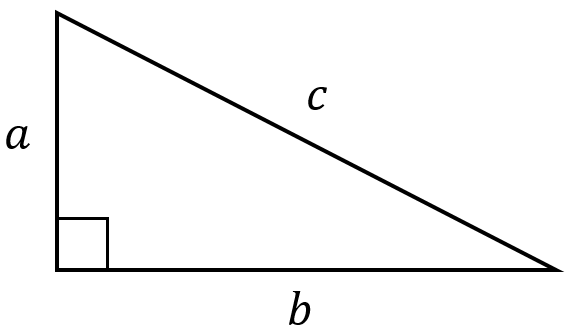
\includegraphics[width=6cm]{trigPythagoras}
		\end{center}
	\end{multicols}
\end{tcolorbox}

This theorem has many proofs, and one graphical one is shown below. The squares are all the same size. Interestingly this proof does not require any math (symbols) at all!

This is a 3-4-5 triangle which is useful in building to determine if something is square: measure sides to 3 and 4 (any units), then check that the hypotenuse is 5.

\begin{figure}
\begin{center}
	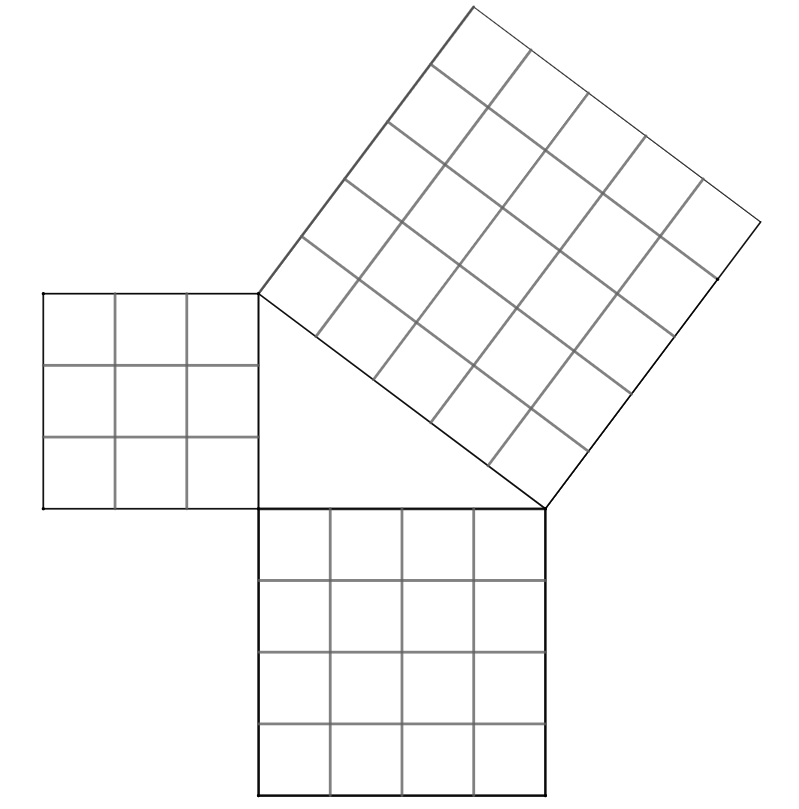
\includegraphics[width=7cm]{PythagorasProof}
\hspace{1cm}
	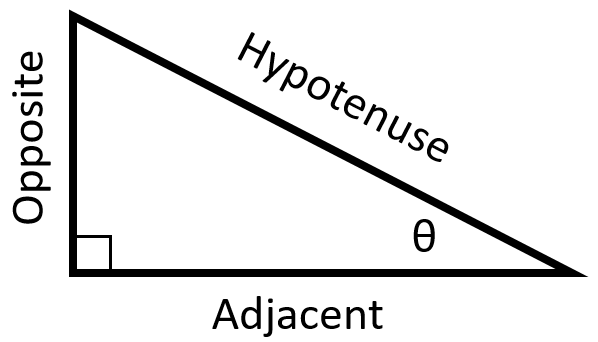
\includegraphics[width=7cm]{rightTriangle}
\end{center}
\end{figure}
\section*{Sine, Cosine, \& Tangent}

The longest side in a right-triangle is always the hypotenuse, with the other two sides being named with respect to the angle of interest, $\theta$. Notice that if $\theta$ moves to the other corner then the sides opposite and adjacent are \textit{reversed}. These names are helpful in defining the trigonometric ratios of sine, cosine and tan.

The phrase \textbf{SOH-CAH-TOA} is useful to remember the ratios.
\begin{tcolorbox}
\begin{equation*}\text{S-ine }  \theta  =\frac{\text{O-pposite}}{\text{H-ypotenuse}}\text{;}\qquad\text{C-osine }  \theta  =\frac{\text{A-djacent}}{\text{H-ypotenuse}}\text{;}\qquad\text{T-angent }  \theta  =\frac{\text{O-pposite}}{\text{A-djacent}}
\end{equation*}\medskip
\hspace{1.7cm}S = O/H\hspace{3.5cm}C = A/H\hspace{3.8cm}T = O/A
\end{tcolorbox}

%----------------------------------------------------
\begin{multicols}{2}
	\example Find the unknown side $x$\\
	\begin{center}
		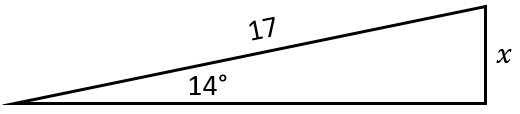
\includegraphics[width=8cm]{trigSide1}
	\end{center}

	\columnbreak
\solution Write the sine ratio and solve the equation for $x$.\\
\begin{align*}
\sin\theta &=\frac{\text{opposite}}{\text{hypotenuse}}\\
\sin (14) &= \frac{x}{17}\\
x&=17\sin(14)\\
x&\approx4.11\end{align*}
\end{multicols}
\rule{6.8cm}{0.5pt}\\
\begin{multicols}{2}
\example Find the unknown side $x$\\
\begin{center}
	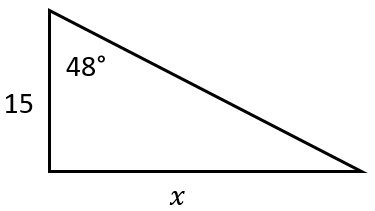
\includegraphics[width=6cm]{trigSide2}
\end{center}
	\columnbreak
\solution Write the tangent ratio and solve the equation for $x$.
\begin{align*}
\tan\theta &=\frac{\text{opposite}}{\text{adjacent}}\\
\tan(48) &= \frac{x}{15}\\
x&=15\tan(48)\\
x&\approx 16.7\end{align*}
\end{multicols}
The calculator gives approximate values of the trigonometric ratios. You must look at your question to check whether angles are in degrees or radians and ensure the calculator is first set in the right mode. Questions where degrees are to be used will give angles marked with a $^\circ$ symbol. 

When solving for an angle on your calculator you select the appropriate trigonometry ratio and use the \emph{shift} button with sin, cos or tan to find $\sin ^{ -1}$, $\cos ^{ -1}$ or $\tan ^{ -1}$. 
%----------------------------------------------------
\begin{multicols}{2}
	\example Find the unknown angle $\theta$\\
	\begin{center}
		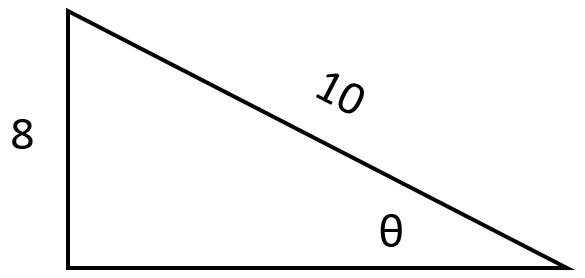
\includegraphics[width=6cm]{trigAngle1}
	\end{center}
	
	\columnbreak
	\solution Write the sine ratio and solve the equation for $\theta$ by using the inverse-trig function on your calculator: $\sin^{-1}$.\\
	\begin{align*}
	\sin\theta &=\frac{\text{opposite}}{\text{hypotenuse}}\\
	\sin \theta &= \frac{8}{10}\\
	\sin\theta&=0.8\\
	\theta&=\sin^{-1}(0.8)\\
	\theta&=\ang{53.1}
	\end{align*}
\end{multicols}\vspace{-0.5cm}
\rule{6.8cm}{0.5pt}\\
\begin{multicols}{2}
	\example Find the unknown angle $\theta$\\
	\begin{center}
		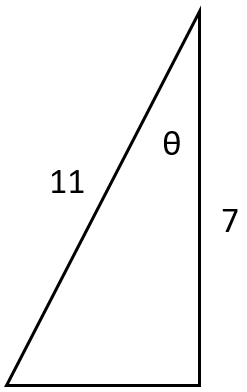
\includegraphics[width=4cm]{trigAngle2}
	\end{center}
	\columnbreak
	\solution Write the cosine ratio and solve the equation for $\theta$ by using the inverse-trig function on your calculator: $\cos^{-1}$.
	\begin{align*}
	\cos\theta &=\frac{\text{adjacent}}{\text{hypotenuse}}\\
	\cos \theta &= \frac{7}{11}\\
	\theta&=\cos^{-1} \left(\frac{7}{11}\right)\\
	\theta&=\ang{50.5}
	\end{align*}
\end{multicols}\vspace{-0.5cm}
%\rule{6.8cm}{0.5pt}\\
%----------------------------------------------------
\example The height of a steep cliff is to be measured from a point on the opposite side of the river. The following diagram shows the measurements taken. Estimate the height of the cliff.
\begin {multicols}{2}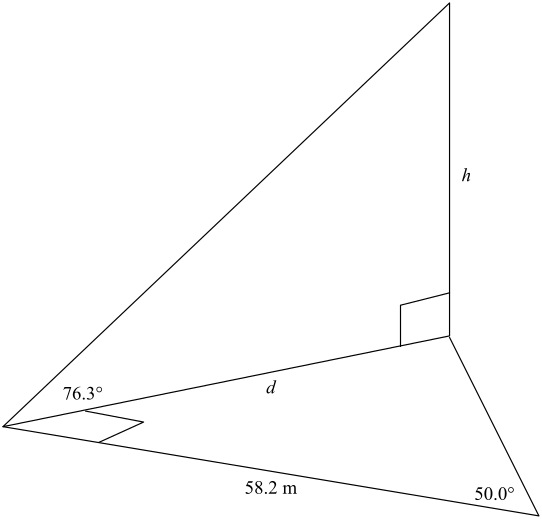
\includegraphics[width=8cm]{L4SZ281H}
%\columnbreak\\
\solution 
\begin{align*}\frac{d}{58.2} &  =  \tan  \ang{50.0}  \\
d &  =  58.2 \times \tan  \ang{50.0}  \\
\frac{h}{d} &  =  \tan  \ang{76.3}  \\
h &  =  d \times \tan  \ang{76.3}  \\
 &  =  58.2 \times \tan  \ang{50.0}  \times \tan  \ang{76.3}  \\
 &  \approx   284.5 \mbox{m}\end{align*}
\end{multicols}

%----------------------------------------------------
\example To estimate the height of a mountain above a level plane the angle of elevation of the top of the mountain is measured to be $\ang{30} $. $600 \mbox{m}$ closer to the mountain across the plane it is found that the angle of elevation is $\ang{36} $. Estimate the height of the mountain. \\
\begin{center}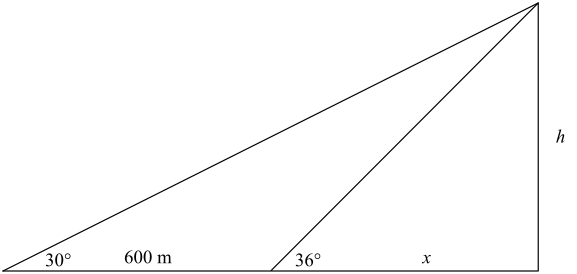
\includegraphics[width=11cm]{L4SZ281I}\end{center}
\solution
\begin{equation*}\frac{h}{x} =\tan  \ang{36} \text{and}\frac{h}{x +600} =\tan  \ang{30} 
\end{equation*}
We want $h$ so we eliminate $x$ between these two equations
\begin{align*}x &  =  \frac{h}{\tan  \ang{36} }\text{and}x +600 =\frac{h}{\tan  \ang{30} } \\
\frac{h}{\tan  \ang{30} } &  =  \frac{h}{\tan  \ang{36} } +600 \\
\frac{h}{\tan  \ang{30} } -\frac{h}{\tan  \ang{36} } &  =  600 \\
h \left (\frac{1}{\tan  \ang{30} } -\frac{1}{\tan  \ang{36} }\right ) &  =  600 \\
h \genfrac{(}{)}{}{}{\tan  \ang{36}  -\tan  \ang{30} }{\tan  \ang{30}  \tan  \ang{36} } &  =  600 \\
h &  =  600 \times \frac{\tan  \ang{30}  \tan  \ang{36} }{\tan  \ang{36}  -\tan  \ang{30} } \\
 &  \approx   600 \times 2.811603815 \\
 &  \approx   1687 \mbox{ m}\end{align*}

%---------------------------------------------------
% identities
%---------------------------------------------------
\subsection*{Identities}\label{sec:identities}
The unit circle has equation $x^{2} +y^{2} =1$ and we define $x =\cos  \theta$ and $y =\sin  \theta$ so
\begin{equation*}x^{2} +y^{2} =1 \leadsto \left (\cos  \theta\right )^{2} +\left (\sin  \theta\right )^{2} =1
\end{equation*}
This is always written
\begin{tcolorbox}\[\sin ^{2} \theta +\cos ^{2} \theta =1\]
\end{tcolorbox}
This is an \emph{identity} which means it is true for all values of $\theta$. There are many identities in trigonometry, we will only use the Pythagorean identity (above) and one more.
Given $\sin =\frac{\text{opp}}{\text{adj}}$ we can solve for $\text{opp}=(\sin)(\text{hyp})$. Similarly from cosine:  $\text{adj}=(\cos)(\text{hyp})$. Substituting these into the tangent relationship:
\begin{tcolorbox}\[\tan=\frac{\text{opp}}{\text{adj}}=\frac{(\sin)(\cancel{\text{hyp}})}{(\cos)(\cancel{\text{hyp}})}=\frac{\sin}{\cos}\]
\end{tcolorbox}
The sine and cosine law are two more unique relationships that we will cover in section~\ref{sec:applications}.

%---------------------------------------------------
% trig functions
%---------------------------------------------------
\subsection*{All Students Take Calculus}
In the previous section the angles were between $\ang{0} $ and $\ang{90} $. In this section the angles can take any value. Initially we consider angles between $\ang{0} $ and $\ang{360} $ and relate these to the radian measure between $0$ and $2 \pi $. We remind you that angles are measured anticlockwise from the positive $x$-axis. 

If the point $P (x ,y)$ is in the first quadrant, $\theta $ is the angle between $OP$ and the positive $x$-axis and we complete the right triangle then we have created the following situation.  

\begin {multicols}{2}
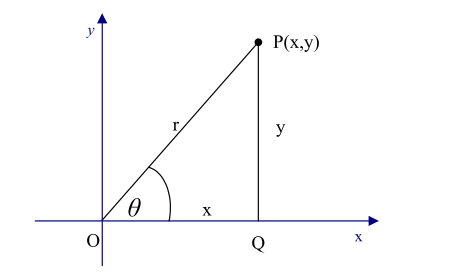
\includegraphics[ width=3.774in, height=2.3454in,]{L4SZ281S}

Let the hypotenuse be $r$ then
\begin{equation*}r =\sqrt{x^{2} +y^{2}}
\end{equation*}
Therefore
\begin{equation*}\sin  \theta  =\frac{y}{r}\text{, }\cos  \theta  =\frac{x}{r}\text{and }\tan  \theta  =\frac{y}{x}
\end{equation*}
\end {multicols}
\begin {multicols}{2}
We now let $\theta $ be any angle and define sine, cosine and tangent in the same way. For instance if $P (x ,y)$ is in the second quadrant: $\sin  \theta  =\frac{y}{r}$ because $y$ is positive $\sin  \theta $ will be positive. ($r$ is always positive.) 

$\cos  \theta  =\frac{x}{r}$ and since $x$ is negative $\cos  \theta $ will be negative. Tangent: $\tan  \theta  =\frac{y}{x}$ and negative for the same reason.\\
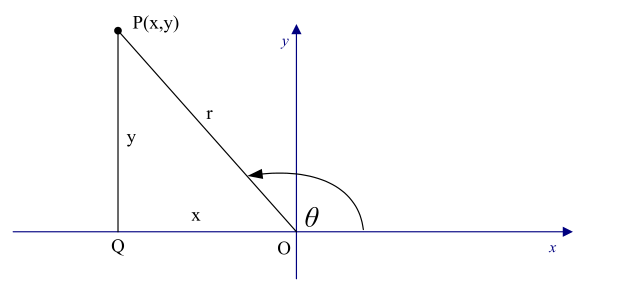
\includegraphics[ width=3.9868in, height=1.8161in,]{L4SZ281T}
\end{multicols}

This pattern can be extended to quadrants 3 and 4. The mnemonic (\textbf{A}ll \textbf{S}tudents \textbf{T}ake \textbf{C}alculus) might help you remember which one is positive although you can always work it out if you need to. This means all are positive in the first quadrant, only sine is positive in the second quadrant, only tangent is positive in the third quadrant and only cosine is positive in the fourth quadrant.

The value of a trigonometric function consists of two parts the numerical part and the sign. you must get both parts correct. In the previous section you related the values of a terminal point to another point in the first quadrant. A point on the unit circle could be in any one of the four quadrants. 

\qquad \qquad \qquad \qquad
\begin{tabular}{cccccc}\toprule
	Quadrant  & $x$-coordinate  & $y$-coordinate  & $\cos $  & $\sin $  & $\tan $  \\\midrule
	I  & $ +$  & $ +$  & $ +$  & $ +$  & $ +$  \\\midrule
	II  & $ -$  & $ +$  & $ -$  & $ +$  & $ -$  \\\midrule
	III  & $ -$  & $ -$  & $ -$  & $ -$  & $ +$  \\\midrule
	IV  & $ +$  & $ -$  & $ +$  & $ -$  & $ -$  \\\bottomrule
\end{tabular}

 

\subsection*{The Area of a Triangle}
The fundamental formula for the area of a triangle is $\text{Area} =\frac{1}{2} \times \text{base} \times \text{height}$ Using the trigonometric functions the height can be replaced and the formula becomes:
\begin{equation*}\text{Area} =\frac{1}{2} \times \text{product of two sides} \times \text{sine of the included angle}
\end{equation*}
The formula is particularly easy to remember in symbolic form. Let the triangle have vertices $A$, $B$ and $C$, so the the sides opposite these angles are $a$, $b$ and $c$ respectively. Then the area can be expressed symbolically as
\begin{equation*}\text{Area} =\frac{1}{2} a b \sin  C =\frac{1}{2} b c \sin  A =\frac{1}{2} a c \sin  B
\end{equation*}

\columnsep =30pt
\begin {multicols}{2} 
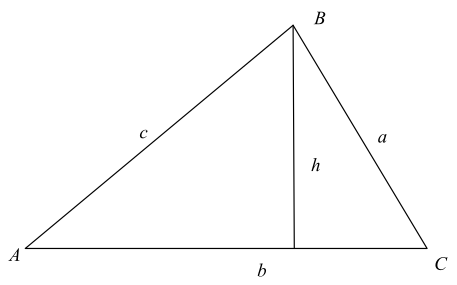
\includegraphics[width=8cm]{L4SZ281U}\label{fig:triangleArea}

\begin{align*}\sin  A &  = \frac{h}{c}\text{ and }h =c \sin  A \\
\text{Area} &  =  \frac{1}{2} \times \text{base} \times \text{height} \\
 &  =  \frac{1}{2} \times b \times c \sin  A =\frac{1}{2} b c \sin  A
 \end{align*}
\end {multicols}
It depends where you draw $h$ and which angle you choose to use as to which formula you finish up with. The key point to remember is $b$ and $c$ are two sides and $A$ is the angle between them. The triangle above shows $A$ as an acute angle (between $\ang{0}$ and $\ang{90} $). If the angle is obtuse (between $\ang{90} $ and $\ang{180} $) the formula still holds. 
\begin{multicols}{2}
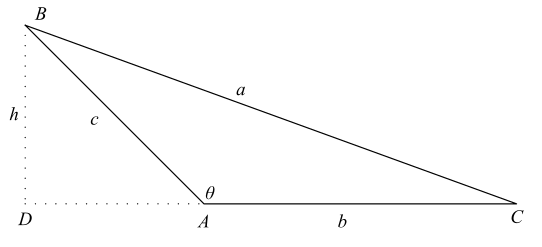
\includegraphics[ width=8cm]{L4SZ281V}
The angle is in the second quadrant and $\sin  (180 -\theta ) =\sin  \theta $, so $\sin  (180 -\theta ) =\frac{h}{c}$ can be written as $\sin  \theta  =\frac{h}{c}$ or $h =c \sin  \theta $ or $h =c \sin  A$ where $A$ is obtuse. So the area is $\frac{1}{2} b c \sin  A$ 
\end{multicols}

\example A triangle has two sides of 5 cm and 8 cm and the angle between them is $\ang{150} $. Find its area.\medskip\\
\solution
\begin{equation*}\text{Area} =\frac{1}{2} \times 5 \times 8 \times \sin  \ang{150} 
\end{equation*}

It helps to remember that $\sin  150 =\sin  30 =\frac{1}{2}$
\begin{equation*}\text{Area} =\frac{1}{2} \times 5 \times 8 \times \frac{1}{2} =10 \text{ cm}^{2}
\end{equation*}

%---------------------------------------------------
% TRIG FUNCTIONS & GRAPHS
%---------------------------------------------------
\section{Trig Functions of Real Numbers}
In this next part of the chapter the three main trigonometric functions (sine, cosine and tangent) will be studied. They will be viewed as functions of real numbers rather than angles. The trigonometric functions defined in these two ways are identical and there is a simple rule connecting the domains. Why do we show you the two approaches? Trigonometry will be used to solve a variety of problems and these can be divided into two groups, dynamic problems and static problems. When dynamic problems (such as problems involving motion) are being solved real numbers will be used. When static problems (such as finding distances and angles for triangles) are being solved angles will be used. 

%---------------------------------------------------
% trig graphs
%---------------------------------------------------
%\section{Trigonometric Functions}
You should be familiar with the fundamental graphs of $y =\sin  x$ and $y =\cos  x$. These graphs are the basis of this section. \Desmos can easily show you the shape of $y =\sin  x$ and $y =\cos  x$ so if you are asked to draw a rough sketch of these curves you should plot a few key points and draw a smooth curve between them. You will usually be given the required domain however if you are not you would choose to draw these for one complete cycle ($0 -2 \pi $). To sketch $y =\sin  x$ it is enough to select as key points $x =0$, $\frac{\pi }{2}$, $\pi $, $\frac{3 \pi }{2}$, $2 \pi $. 

\begin{center}
\begin{tabular}{llllll}\toprule
	$x$  & $0$  & $\dfrac{\pi }{2}$  & $\pi $  & $\dfrac{3 \pi }{2}$  & $2 \pi $ \\\midrule
	$y =\sin  x$  & $0$  & $1$  & $0$  & $ -1$  & $0$  \\\bottomrule
\end{tabular}
\hspace{1cm}
\begin{tabular}[c]{llllll}\toprule
	$x$  & $0$  & $\dfrac{\pi }{2}$  & $\pi $  & $\dfrac{3 \pi }{2}$  & $2 \pi $ \\\midrule
	$y =\cos  x$  & $1$  & $0$  & $ -1$  & $0$  & $1$ \\\bottomrule
\end{tabular}
\end{center}

You will be aware that these curves repeat this pattern every $2 \pi $ where $x$ extends in both the positive and negative directions. $0$ to $2\pi $ represents one complete cycle. Mathematically we say
\begin{align*}\sin  \left (x +2 n \pi \right ) &  = \sin  x\text{\  for any integer }n \\
	\cos  \left (x +2 n \pi \right ) &  = \cos  x\text{\  for any integer }n\end{align*}

Aside: instead of ``for any integer $n$" we can write $ \forall n \in \mathbb{Z}$. A function that displays this characteristic is described as \emph{periodic} and for $y =\sin x$ and $y =\cos x$ the \emph{period} is $2 \pi $. 

\subsection*{Transformations}
The following six transformations can be applied to any function including sine, cosine, and tangent. 
\begin{tasks}[style=itemize](3)
\task Vertical shift 
\task Horizontal shift 
\task Vertical stretch 
\task Horizontal stretch 
\task Reflection in the $x$-axis 
\task Reflection in the $y$-axis 
\end{tasks}

\example Sketch $y =\sin  \left (x -\frac{\pi }{2}\right ) +3$. This may be considered as a sine curve shifted $\frac{\pi }{2}$ units to the right. Note for periodic functions like a sine wave a horizontal shift is called a \textit{phase shift}. and $3$ units upwards.\\ 
\solution 1. Beginning with the special points for $\sin x$, a table shows the evolution of the points. \\
\begin{tabular}{llllllc}\cmidrule{1-6}
	$x$  & $0$  & $\frac{\pi }{2}$  & $\pi $  & $\frac{3 \pi }{2}$  & $2 \pi $ & $\leftarrow x$-values, plot these \\
	\cmidrule{1-6}
	$\sin  x$  & $0$  & $1$  & $0$  & $ -1$  & $0$ & \\
	\cmidrule{1-6}
	$\sin  \left (x -\frac{\pi }{2}\right )$  & $ -1$  & $0$  & $1$  & $0$  & $ -1$&  \\
	\cmidrule{1-6}
	$\sin  \left (x -\frac{\pi }{2}\right ) +3\qquad$  & $2$  & $3$  & $4$  & $3$  & $2$&$\leftarrow y$-values, plot these  \\
	\cmidrule{1-6}
\end{tabular}

2. Plot the transformed values with the original special points and connect with a smooth, continuous line. \Desmos confirms our transformation. The dashed plot shows $y=\sin x$ as reference.\\
\begin{center}
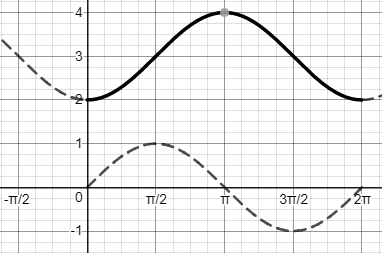
\includegraphics[width=8cm]{trigShift1}
\end{center}


\example Sketch $y =\cos  (x -\frac{\pi }{6})$.\medskip\\
\solution You could use a table of values however this is $y =\cos  x$ with a horizontal shift of $\frac{\pi }{6}$ to the right. Sketch the transformation on top of the graph of $y =\cos  x $.
\begin{center}
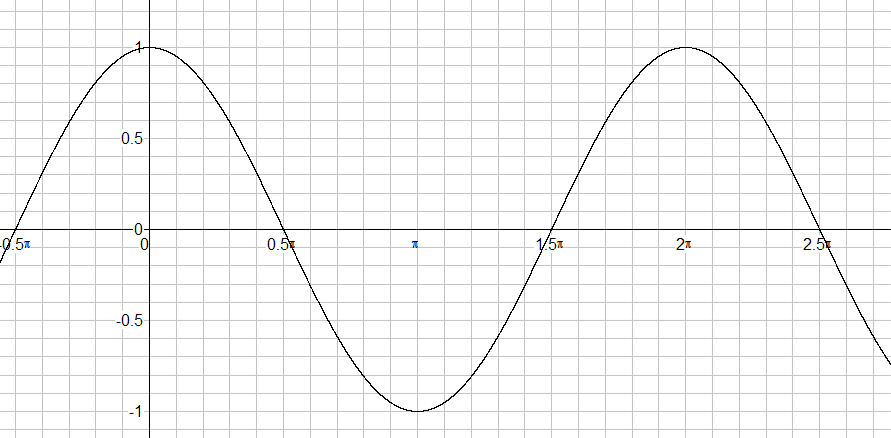
\includegraphics[width=10cm]{L4SZ270H}
\end{center}

In general $y =a \sin  x$ represents a vertical stretch of $y =\sin  x$ by $a$. If $a$ is negative the transformation can either be described as a negative stretch or (preferably) as a \emph{stretch}
of $\left \vert a\right \vert $ followed by a \emph{reflection} in the $x$-axis. Recall the reflection of $y =f \left (x\right )$ in the $x$-axis is $y = -f \left (x\right )$. The number $\left \vert a\right \vert $ is called the \emph{amplitude} for both $y =\sin  x$ and $y =\cos  x$ shown below. 

If $0 <a <1$ the fractional stretch causes the curve to shrink vertically. For instance the curve
$y =\sin  x$ has a maximum value of $1$ and a minimum value of $ -1$. the curve $y =\frac{1}{2} \sin  x$ has a maximum value of $\frac{1}{2}$ and a minimum value of $ -\frac{1}{2}$. 

\begin{tasks}(2)
\task\example Sketch $y =\cos  ( -t)$ \medskip\\
Notice this reflection is on top of the original. Cosine is symmetric about the $y$-axis.\\
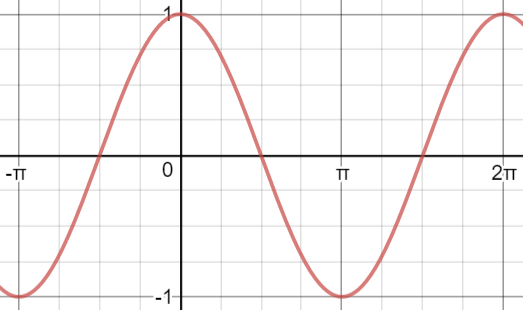
\includegraphics[width=8cm]{trigTrans1}\\

\task\example Sketch $y =\sin(x+\frac{\pi}{4})$\medskip\\
The angle is shifted to the left by 45 degrees ($\frac{\pi}{4}$ radians).\\
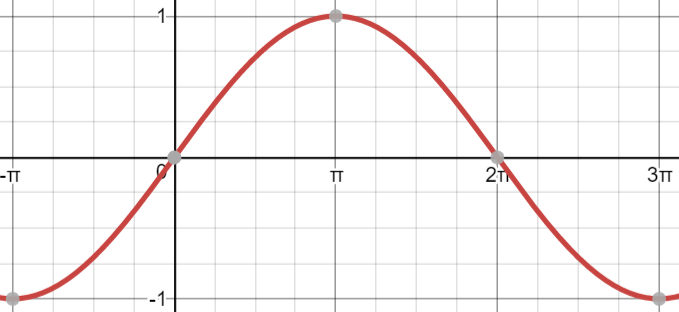
\includegraphics[width=8cm]{trigTrans2}

\task\example Sketch $y =\cos(2x)$ \medskip\\
Here there are 2 complete cycles between 0 and $2\pi$.\\
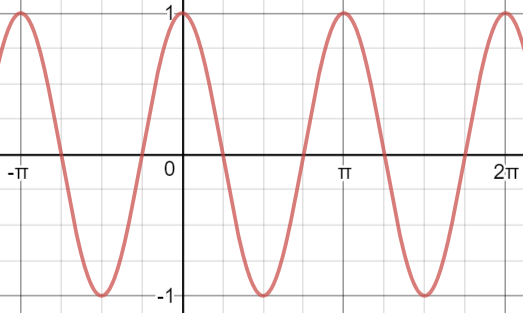
\includegraphics[width=8cm]{trigTrans3}

\task\example Sketch $y =2\sin(0.5x)$ \medskip\\
Two transformations applied together. The 2 refers to the amplitude.\\
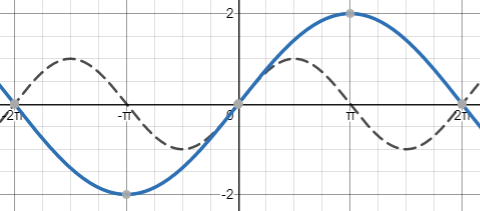
\includegraphics[width=8cm]{trigTrans4}
\end{tasks}

\subsection*{Tangent}
 There are other trig functions that we will not be covering here, for example the reciprocal functions are cosecant$=\frac{1}{\sin\theta}$, secant$=\frac{1}{\cos\theta}$, and the inverse tangent function, cotangent$=\frac{1}{\tan\theta}$. By focussing on sine, cosine and tangent the majority of problems we encounter can be solved. Tangent is the odd function out of the trio of common ones.

Previously we learnt that the period for the sine and cosine functions was $2 \pi $. Tangent is also a periodic function and it has a period of $\pi $ (not $2 \pi $). This means that it goes through one complete cycle every $\pi$. Recall $\tan  x =\frac{\sin  x}{\cos  x}$. To analyse the behaviour of the tangent function it helps if you know what you are looking for. Some key values of tangent will show the pattern. 
\begin{center}
\begin{tabular}{lrrrl}\toprule
	$x$  & $\qquad\sin  x$  & $\qquad\cos  x$  &\qquad\quad& $\tan  x$  \\
	\midrule
	$ -\frac{\pi }{2}$  & $ -1$  & $0$  && $\frac{ -1}{0} = -\infty $  \\
	\midrule
	$ -\frac{\pi }{4}$  & $ -\frac{\sqrt{2}}{2}$  & $\frac{\sqrt{2}}{2}$  && $ -\frac{\sqrt{2}}{2} \div \frac{\sqrt{2}}{2} = -1$  \\
	\midrule
	$0$  & $0$  & $1$  && $\frac{0}{1} =0$  \\
	\midrule
	$\frac{\pi }{4}$  & $\frac{\sqrt{2}}{2}$  & $\frac{\sqrt{2}}{2}$  && $\frac{\sqrt{2}}{2} \div \frac{\sqrt{2}}{2} =1$  \\
	\midrule
	$\frac{\pi }{2}$  & $1$  & $0$  && $\frac{1}{0} =\infty $  \\
	\bottomrule
\end{tabular}
\end{center}
As $x$ takes values from $ -\frac{\pi }{2}$ to $\frac{\pi }{2}$, $\tan(x)$ takes values from $ -\infty $ to $\infty $. This pattern is repeated every $\pi $. 
A \desmos graph can show this relationship. The dashed lines are the asymptotes.

\begin{figure}\begin{center}
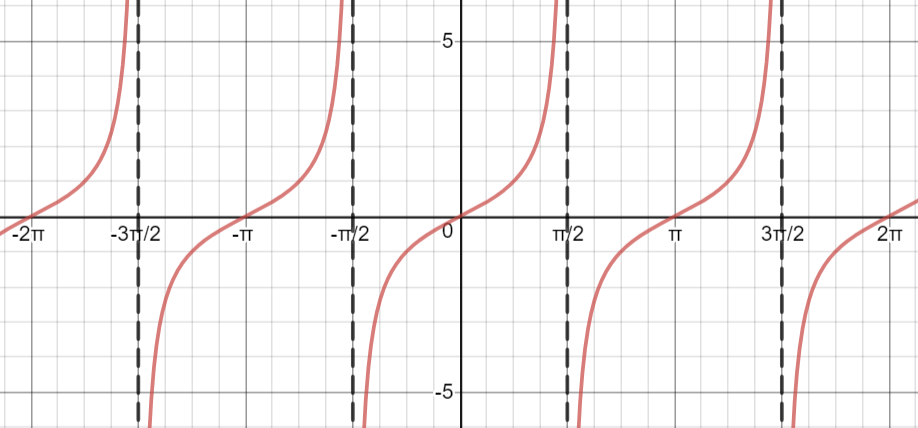
\includegraphics[width=12cm]{trigTan}
\caption{The graph of $y=\tan x$. The asymptotes are shown with dashed lines, repeating every $\pi$ radians.}
\end{center}\end{figure}

The graph can be seen to have point symmetry. If you rotate the tangent curve through a half turn using the origin as axis the curve will lie on top of itself. This is a pictorial representation of an odd function.

Note: Do not confuse $y =\tan  x$ with $y =x^{3}$. While they may appear to be similar in shape the only similarities are that they both pass through the origin and continue towards $\infty $ in the first quadrant and $ -\infty $ in the third quadrant. 

%---------------------------------------------------
% sine rule and cosing rule
%---------------------------------------------------
\section{Applications}\label{sec:applications}
\subsection*{The Sine Rule}
The Sine Rule is a relationship that allows you to find the sides and angles in triangles \textit{without} a right angle. In the next section we use the Cosine Rule to find sides and angles in triangles also, so as you study these two sections you need to learn which problems require the Sine Rule and which require the Cosine Rule. Previously, we met the formula for the area of a triangle given two sides and the included angle $\left ( \text{area}=\frac{1}{2} a b \sin  C\right )$. The Sine Rule and Cosine Rule also require specific combinations of sides and angles. Using standard side and angle labelling for a triangle $\rightarrow$ $\Delta A B C$ and let the sides be lowercase $a$, $b$ and $c$ where $a$ is opposite $\angle A$ etc. 
\begin{center}
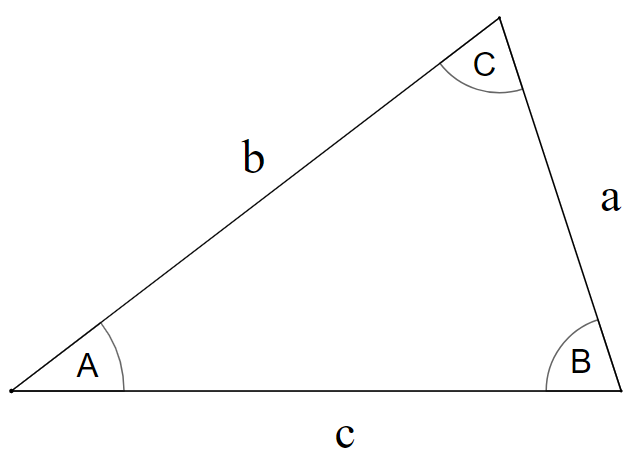
\includegraphics[width=7cm]{SineRuleTriangle1}
\end{center}

\begin{tcolorbox}
	The Sine Rule states that in any triangle
	\begin{equation*}\frac{\sin  A}{a} =\frac{\sin  B}{b} =\frac{\sin  C}{c}\qquad%
	\text{ or, inversely as: }%
	\qquad\frac{a}{\sin  A} =\frac{b}{\sin  B} =\frac{c}{\sin  C}
	\end{equation*}\end{tcolorbox}
Textbooks may use the term ``The Law of Sines'' meaning the same relationship. 

\subsection*{Proof of the Sine Rule}
The Sine Rule is easy to prove beginning with the formula for the area of a triangle, and using the diagram above as reference with the base as $c$. (Refer to the diagram on page~\pageref{fig:triangleArea}.)
\begin{equation*}\text{Area} =\frac{1}{2}(\text{base})(\text{height})=\frac{1}{2} (c)(b\sin A)=\dots=\frac{1}{2}ab\sin C=\frac{1}{2}ac\sin B
\end{equation*}
Focussing only on the three terms on the right, multiply by 2:
\begin{equation*}b c \sin  A=ab\sin C=ac\sin B
\end{equation*}

And dividing by $a b c$
\begin{equation*}\frac{\sin A}{a}=\frac{\sin B}{b}=\frac{\sin C}{c}
\end{equation*}
\clearpage
%\rule{\textwidth}{0.5pt}\\
\begin{multicols}{2}
\example Find side lengths $a$ and $c$ in the following triangle.\\
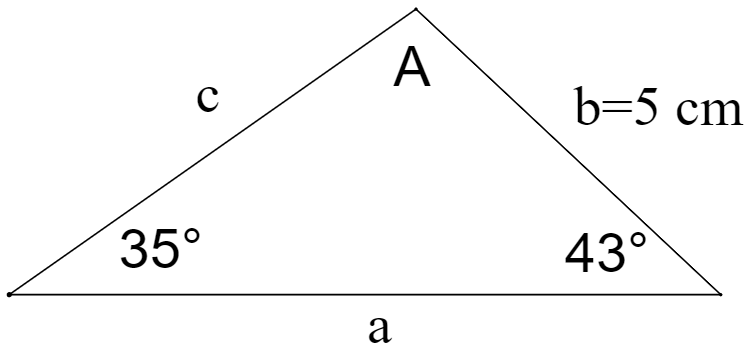
\includegraphics[width=8cm]{SineRuleTriangle2}\\
$\phantom{1}$\\
$\phantom{1}$\\
\solution \medskip\\(1) To find $c$
\begin{align*}\frac{c}{\sin  C} &  = \frac{b}{\sin  B} \\
\frac{c}{\sin  43 } &  = \frac{5}{\sin  35 } \\
c &  = \frac{5 \sin  43 }{\sin  35 } \\
&  \approx   5.95 \mbox{cm}\text{(2 dp)}\end{align*} \\
%\clearpage
(2) To find $a$ (i) $A =\ang{180}  -(\ang{35}  +\ang{43} ) =\ang{180}  -\ang{78}  =\ang{102}$ (ii) It is usually wise to go back to the original data (i.e. use $b$ and $B$ rather than $c$ and $C$).
\begin{align*}\frac{a}{\sin  A} &  = \frac{b}{\sin  B} \\
\frac{a}{\sin  102 } &  = \frac{5}{\sin  35 } \\
a &  = \frac{5 \sin  102 }{\sin  35 } \\
&  \approx   8.53 \mbox{cm}\text{(2 dp)}\end{align*}
\end{multicols}

These two calculations illustrate the first two cases in which the Sine Rule is used. You will notice that the triangle has been completely solved in the course of this example. We started with one side and two angles and we found the other two sides and the other angle. \\
\rule{6.8cm}{0.5pt}\\
\example Given $a =\ang{30} $, $a =8$ and $b =7$ solve the triangle (i.e. find $B$, $C$ and $c$). \\
\begin{center}
	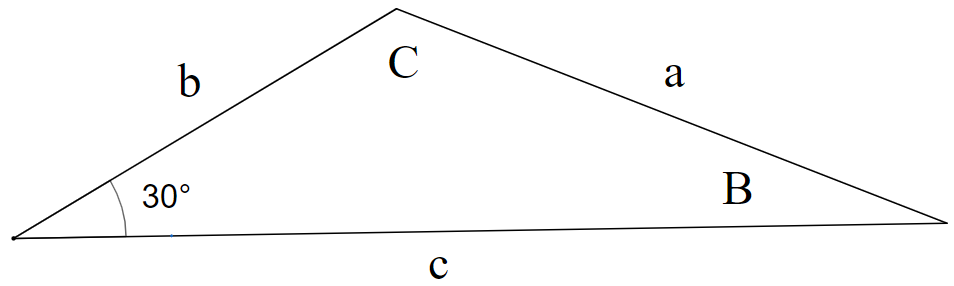
\includegraphics[width=11cm]{SineRuleTriangle3}\\
\end{center}
\solution
\begin{tasks}[counter-format=(tsk[1]),before-skip = {0ex},after-skip={-5ex}](3)
\task Find $B$
\begin{align*}\frac{\sin  B}{b} &  = \frac{\sin  A}{a} \\
\sin  B &  = \frac{b \sin  A}{a} \\
&  = \frac{7 \sin  30 }{8} =0.4375 \\
B &  = \sin ^{ -1} 0.4375 \approx \ang{25.94} \end{align*}

\task Find $C$
\begin{align*}C &  = \ang{180}  -(\ang{30}  +\ang{25.94} ) \\
&  = \ang{124.06} \end{align*}

\task Find $c$
\begin{align*}\frac{c}{\sin  C} &  = \frac{a}{\sin  A} \\
c &  = \frac{a \sin  C}{\sin a} \\
&  = \frac{8 \sin  124.06 }{\sin  30 } \\
&  \approx   13.3\end{align*}
\end{tasks}
%--------ambiguous case example---------------------------
The third case is not as straight forward and referred to as the ambiguous case. Given two sides and an angle there could be no triangle formed, one triangle formed or two triangles formed depending on the length of the side opposite the given angle.

\example {The Ambiguous Case:} Given $A =\ang{30} $, $a =6$ and $b =7$ solve the triangle. \\

\solution In this case $b \sin  A =3.5$ and $b =7$ so as $a$ lies between $3.5$ and $7$. This is the ambiguous case, therefore there are two solutions as the side lengths and angle can produce two different triangles.
%\columnsep =30pt
\begin {multicols}{2}
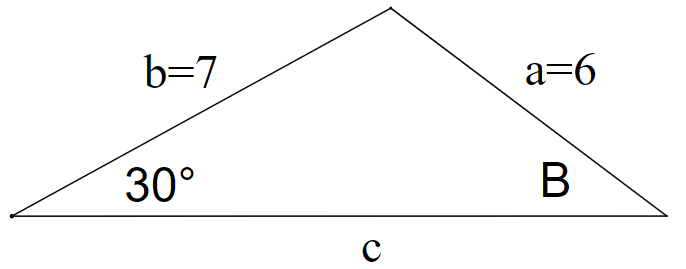
\includegraphics[width=8cm]{SineRuleAmb1}\columnbreak
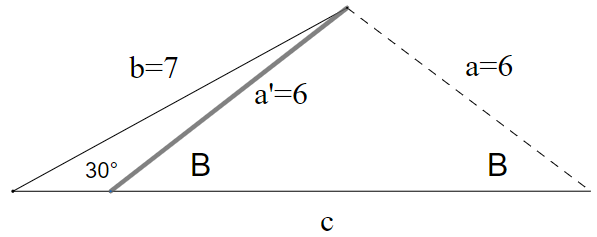
\includegraphics[width=8cm]{SineRuleAmb2}
\end {multicols}
\textbf{First solution} (Proceed as before) 
\begin{tasks}[counter-format=(tsk[1]),before-skip = {0ex},after-skip={-5ex}](3)
	\task Find $B$
\begin{align*}\frac{\sin  B}{b} &  = \frac{\sin  A}{a} \\
\sin  B &  = \frac{b \sin  A}{a} \\
&  = \frac{7 \sin  30 }{6} =0.58 \dot{3} \\
B &  = \sin ^{ -1} 0.58 \dot{3} \approx \ang{35.7} \end{align*}

\task Find $C$\\
First recognize this angle is obtuse $>\ang{90}$
\begin{align*}C &  = \ang{180}  -(\ang{30}  +\ang{35.69} ) \\
&  = \ang{114.31} \end{align*} 

\task Find $c$
\begin{align*}\frac{c}{\sin  C} &  = \frac{a}{\sin  A} \\
c &  = \frac{a \sin  C}{\sin  A} \\
&  = \frac{6 \sin  114.31 }{\sin  30 } \\
&  \approx   10.9\end{align*}
\end{tasks}
\textbf{Second solution} 
\begin{tasks}[counter-format=(tsk[1]),before-skip = {0ex},after-skip={-5ex}](2)
	\task Find the second value of $B$ \\
$B =\ang{180}  -\ang{35.69}  =\ang{144.31} $
\task Find $C$\\
$C =\ang{180} -(\ang{30}  +\ang{144.31} ) =\ang{180}  -\ang{174.31}  =\ang{5.69} $
\task*[](Or if you remember the rule that the exterior angle of a triangle is the sum of the two interior opposite angles $C +\ang{30}  =\ang{35.69} $ so $C =\ang{35.69}  -\ang{30}  =\ang{5.69} $) 
\task[(3)] Find $c$
\begin{align*}\frac{c}{\sin  C} &  = \frac{a}{\sin  A} \\
c &  = \frac{a \sin  C}{\sin  A} \\
&  = \frac{6 \sin  5.69 }{\sin  30 } \\
&  \approx   1.2\end{align*}
\task[]Both answers here are correct mathematically, however, depending on the situation one answer refers to a specific triangle which should be checked with a diagram.
\end{tasks}

\subsection*{The Cosine Rule}
In this section we will state and prove the Cosine Rule (which is called "The Law of Cosines" in the textbook). The proof is given here for completeness. You will not be tested on your ability to reproduce it. The section will give examples where the Cosine Rule is used to solve problems using the \emph{triangle of vectors} and we will include revision of \emph{bearings} and the use of trigonometry in \emph{navigation}. 

\begin{tcolorbox}
	For any triangle side sides $a$, $b$, and $c$ and angle $A$ opposite side $a$:\\
	\begin{center}
		$a^{2} =b^{2} +c^{2} -2 b c \cos  A$
	\end{center}	
\end{tcolorbox}

\subsection*{Proof of The Cosine Rule}
\textbf{To prove:} For any triangle $ \Delta A B C\text{,}$ $a^{2} =b^{2} +c^{2} -2 b c \cos  A$ \\ 
\columnsep =30pt
\begin {multicols}{2}
\setlength\fboxrule{0in}\setlength\fboxsep{0.2in}\fcolorbox[HTML]{000000}{FFFFFF}{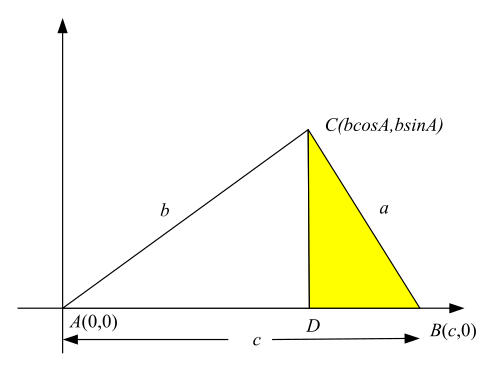
\includegraphics[ width=3.1021in, height=2.3549in,]{L4SZ282A}}
By Pythagoras' Theorem
\begin{align*}B C^{2} &  = C D^{2} +D B^{2} \\
a^{2} &  = \left (c -b \cos  A\right )^{2} +\left (b \sin  A\right )^{2} \\
&  = c^{2} -2 b c \cos  A +b^{2} \cos ^{2} A +b^{2} \sin ^{2} A \\
&  = c^{2} -2 b c \cos  A +b^{2} \left (\cos ^{2} A +\sin ^{2} A\right ) \\
&  = c^{2} -2 b c \cos  A +b^{2}\text{as}\cos ^{2} A +\sin ^{2} A =1\text{\ }\end{align*} 
\end {multicols}
This is usually written
\begin{equation*}a^{2} =b^{2} +c^{2} -2 b c \cos  A
\end{equation*}

The diagram has been drawn to simplify the way the proof unfolds. You will see that by placing the vertex $A$ at the origin the side $a$ is found in terms of $b$, $c$, and $A$. The proof would have been the same had $A$ and $B$ been as shown and $C$ placed in the second quadrant. (Thus producing a triangle with an obtuse angle at $A$.) This rule is symmetrical. You need to be given two sides and the included angle ($b$, $c$ and $A$) and the formula allows you to calculate $a$. Most textbooks will therefore show you three equivalent formulae:
\begin{align*}a^{2} &  = b^{2} +c^{2} -2 b c \cos  A \\
b^{2} &  = c^{2} +a^{2} -2 c a \cos  B \\
c^{2} &  = a^{2} +b^{2} -2 a b \cos  C\end{align*}
\rule{6.8cm}{0.5pt}\\
\example Given $a =5$, $b =6$ and $C =\ang{130} $, find $c$.\medskip\\
\solution
\begin{align*}c^{2} &  = a^{2} +b^{2} -2 a b \cos  C \\
&  = 5^{2} +6^{2} -2 \times 5 \times 6 \times \cos  130  \\
c^2&  \approx   99.567 \\
c &  \approx   \sqrt{99.567}  \approx   9.978\end{align*}

\example Find the angle given three side lengths; given $a =5$, $b =6$ and $c =9$, find $A$. \medskip\\
\solution Because $a$ is the smallest side $A$ will most certainly be an acute angle.
\begin{align*}\cos  A &  = \frac{b^{2} +c^{2} -a^{2}}{2 b c} \\
&  = \frac{6^{2} +9^{2} -5^{2}}{2 \times 6 \times 9} \\
&  \approx 0.852 \\
A &  \approx \cos ^{ -1} \left (0.852\right ) \\
&  \approx \ang{31.6} 
\end{align*}

%---------------------------------------------------
% Chapter Exercises in a separate file
%---------------------------------------------------
\section{Chapter Exercises}
\subimport{}{2TrigExercises}

